%\documentclass{article}
\documentclass[preprint,aip,pra]{revtex4-1}
\usepackage{hyperref}
\usepackage{amsmath}
\usepackage{csquotes}
\usepackage{gensymb}
\usepackage{graphicx}
\graphicspath{ {images/} }
\usepackage{physics}
\usepackage{color}
\newcommand{\red}[1]{\textcolor{red}{\bf #1}}

\begin{document}

\title{Nuclear Wastes: we're kinda doomed}

\author{Yuping Huang}%
\affiliation{Department of Physics and Astronomy, Carleton College}

\date{\today}%
\begin{abstract}
    meep
\end{abstract}
\maketitle
\tableofcontents
\newpage

\section{Introduction}
IAEA nuclear waste estimation: over 1000 tons of highly radioactive waste.\cite{iaea08}
Nuclear power estimate:increase by 40\% by 2020. \cite{iaea12}
meep. Mostly focus on nuclear waste from reactors.
Global policy review \cite{r12} 

Where they come from:\\
mop

what to do with them:\\
meep

\begin{itemize}
    \item history
    \item nuclear decay mechanism: weak force and tunneling, radioactive decay
    \item reactors?
    \item What is nuclear waste and why is it harmful?
    \item partition and transmutation
    \item Above-ground disposal: look at sites, dry-casks storage
    \item geological disposal ($\star$), Yucca mountain as an example
    \item ocean floor disposal which was done by everyone but not legal any more
    \item transmutation
    \item todo: find sources on the specific health impact of nuclear waste instead of radiation
        in general
\end{itemize}

\section{Radioactivity and nuclear fission}
    Here we detail the nuclear physics underlying most of the things we will talk about
    in this work. We will apply these results in our discussion of nuclear wastes.
    \subsection{Radioactivity}
    \subsubsection{Nuclear shell model vs liquid drop model(?)}
        By solving Schr\"{o}dinger's equation\cite{k88}
    \subsubsection{Binding Energy(?)}

        \subsubsection{Quantum theory of radioactive decays}
        We have learned that radioactivity is stochastic in nature and radioactive decay follows
        an exponential law
        \begin{equation} \label{eq:exp}
            \lambda = -\frac{(dN/dt)}{N},
        \end{equation}
        where $\lambda$ is the decay constant, and the right hand side the probability of decay
        per time for an atom. The fundamental assumption is that the probability of decay is constant,
        regardless of the age of the atom. This ``memorylessness'' assumption naturally leads to the
        exponential law of radioactive decay
        \begin{equation}
            N(t) = N_0 e^{-\lambda t},
        \end{equation}
        where $N_0$ gives the number of nuclei at $t=0$.

        Define activity $\mathcal{A}(t)$ to be the rate of decays in a sample
        \begin{equation} \label{eq:act}
            \mathcal{A}(t)\equiv \lambda N(t).
        \end{equation}
        Here we outline an quantum mechanics argument for an exponential decay law that is perhaps more
        convincing.
        We approximate the potential by $V+V_p$ where $V$ is the nuclear potential and $V_p$ is a small
        time-dependent perturbation that causes the transition between the states. We know that there has
        to be time dependence in the potential, otherwise for a superposition of eigenstates
        $\ket{psi}=c_1\ket{\psi_1} + c_2\ket{\psi_2}$, the coefficients $c_1$ and $c_2$ would 
        have to be constant and
        persistent decay of one state into the other would not happen.
        Fermi's Golden Rule \#2 (which is derived in appendix \ref{a:fermi})
        gives the transition rate
        \begin{equation}
            \label{eq:trans}
            \lambda = \frac{2\pi}{2\hbar}|\bra{\psi_f}V_p\ket{\psi_i}|^2\rho(E_f),
        \end{equation}
        where $\ket{\psi_i}$ denotes the initial state , $\bra{\psi_f}$ the final state, $V_p$ the perturbation
        potential and $\rho(E_f)$ the density of state of the final state, defined by
        \begin{equation}
            \rho(E_f) = \frac{dn_f}{dE_f}.
        \end{equation}
        Note that as in perturbation theory, $\ket{\psi_i}$ and
        $\ket{\psi_f}$ are both eigenstates of the nuclear potential $V$. Therefore, as long as
        the decay probability is small, the result from perturbation theory should hold. Since
        there is no time dependency in equation~\ref{eq:trans},the
        decay rate should be independent of time, which is the fundamental assumption made in
        equation~\ref{eq:exp}.

        \subsubsection{Quantifying radioactivity}
        The radioactivity of a sample $\mathcal{A}$ (defined in equation~\ref{eq:act}) 
        is the number of decays of the sample per unit time. The SI
        unit for radioactivity is becquerel (Bq) and it equals one decay per second. Another commonly used
        unit is curie (Ci, with $1\text{ Ci}=3.7\times 10^{10}\text{ Bq}$) and it is defined as
        the activity of radium-266. A fission product, cesium-137 has an activity of $3.215\times 10^{12}$ Bq
        per gram. By contrast, the radioactivity of a human body (mainly due to the small amount of 
        potassium-40 and carbon-14) is about $8000$ Bq.

    \subsection{Biological Effects of Radiation}
        The biological effects of radiation have been an important topic for decades. A large
        number of studies took place after the two nuclear bomb explosions in Japan in 1945
        and after disastrous nuclear plant accidents like Chernobyl. Therefore, we have a relatively
        thorough understanding of the consequences of mass exposure to radiation. However, relatively
        little is known about the long-term effects of exposure to small doses, including subtle biological
        changes that lead to cancer and genetic defects. Here we briefly summarize the known effects.
        \subsubsection{Different kinds of radiation and shielding}
        meep
        \subsubsection{Quantifying radiation on living tissues}
        The biological impact of radiation depends on the type, power and energy of the radiation, the
        exposure time, and the part of the body exposed. Various quantities have been introduced to
        measure the amount of radiation and the biological impact of radiation. Here we review three
        of these quantities: the absorbed dose, the equivalent dose and the effective dose.

        The amount of radiation is usually characterized by the amount of energy it carries. Since one of
        the earliest understood effects of radiation is its ability to ionize gas, one can quantify the
        strength of the radiation with the ionizing energy of the gas.
        Absorbed dose~($D$) quantifies the 
        radiation energy absorbed per unit mass. The modern unit is Gray(Gy)
        and $1\text{Gy}=1\text{J kg}^{-1}$.\cite{u16}

        Biological effects not only depend on the total dose applied but also the rate at which the 
        dose is applied, because mechanisms exist within organisms that allow molecules like deoxyribonucleic acid
        to be repaired if they are not excessively damaged. Therefore {\it dose rate} is also a useful
        measure of radiation when considering its biological effect.

        For an external $\gamma$-ray source emitting $\mathcal{A}$ million photons per second 
        of energy $E_{\gamma}$
        (in MeV), one can approximate the dose rate by 
        \begin{equation}
            \frac{dD}{dt}(\mu\text{Sv h}^{-1}) \approx \frac{\mathcal{A}\text{(MBq)}\times E_{\gamma}\text{(MeV)}}
            {6\times [r\text{(m)}]^2}.
        \end{equation}
        The approximate\red{(?)} linear dependence on $E_{\gamma}$ is valid from less than $0.1$ MeV to several
        MeV and therefore should be good for all sources but those generated in an accelerator.\cite{my68}
        The inverse-squared dependence on distance is hardly surprising.

        However, absorbed dose does not take into account different biological implications of different types
        of radiation.
        For example, the same dose of alpha particle can do more damage to body than gamma rays. The equivalent
        dose ($H$) is defined as
        \begin{equation}
        H=w_R \times D_R,
        \end{equation}
        where $D_R$ is the absorbed dose and $w_R$ the weighting factor of a given kind of radiation $R$
        (see table \ref{tab:eq} for a list of weighing factors). If there are multiple types of radiation 
        present, the equivalent does is given by the weighted sum over all contributions. The SI unit for
        equivalent dose is called the sievert (Sv) and $1\text{ Sv}=1\text{ J kg}^{-1}$.
        \\\red{Dose distribution and bio effectiveness?}
        \begin{table}
            \label{tab:eq}
            \centering
            \caption{Weighting factors for different types of radiation\cite{icrp74}}
            \begin{ruledtabular}
                \begin{tabular}{l c c}
                Type of radiation & Energy range & Weighting factor, $w_R$\\
                \hline
                Photons, electrons & All energies & 1\\
                Neutrons & $<10$ keV & 5 \\
                         & $10-100$ keV & 10 \\
                         & $100$ keV-$2$ MeV & 20 \\
                         & $2-20$ MeV & 10 \\
                Protons & $<20$ MeV & 5 \\
                Alpha particles, fission fragments, heavy nuclei & & $20$\\
            \end{tabular}
            \end{ruledtabular}
        \end{table}
        Finally, certain organs and parts of the body are more vulnerable to radiation than the rest.
        Therefore, effective dose~($E$) is defined as the equivalent dose weighted by the body part
        radiated
        \begin{equation}
            E = w_T H_T,
        \end{equation}
        where $w_T$ is the body tissue weighting factor, and $H_T$ the equivalent dose on the tissue
        at question.
        Evidently, if the radiation affects multiple tissues, the effective dose will be the weighted
        sum of the equivalent dose over individual body parts. Some of the recommended values of tissue
        weighting factors are given in table \ref{tab:eff}. A weighing factor of $1$ is equivalent to the
        whole body absorbing the radiation uniformly. The SI unit of effective dose is sievert (Sv),
        identical to that of equivalent dose.
        \begin{table}
            \label{tab:eff}
            \centering
            \caption{Weighting factors for individual organs\cite{icrp74}}
            \begin{ruledtabular}
                \begin{tabular}{l c}
                Tissue & Weighting factor, $w_T$\\
                \hline
                Gonads & $0.20$\\
                Red bone marrow & $0.12$ \\
                Liver & $0.05$ \\
                Skin & $0.01$ \\
                \end{tabular}
            \end{ruledtabular}
        \end{table}
        \subsubsection{Effects of radiation on human}
        Short-term effects of radiation are usually caused by extensive cell death or cell damage.\cite{u16}
        These effects are deterministic, meaning that below a certain threshold the effect does not occur and
        the severity of the effect depends on the dose. Some examples are gastrointestinal damage and impairment
        of fertility.\cite{u16, l01}

        Delayed health effects occur a long time after the exposure and are usually stochastic. There is
        no apparent threshold and the severity is usually independent of the dose but
        the chance of occurrence depends on the dose.\cite{u16,l01}
        For example, according to a review done by the UN Scientific Committee on the Effects of Atomic Radiation
        (UNSCEAR), the additional chance of dying of cancer due to radiation exposure above $100$ mSv is
        about 3 to 5 percent per sievert.\cite{unscear12}
        \red{LNT vs threshold?}

        Hereditary effects of radiation can occur if the reproduction cells were damaged by radiation.
        UNSCEAR estimates that risk for severe hereditary effect is about $0.3-0.5$ percent per gray to
        the first generation following the radiation exposure.\cite{u16, unscear12}

        \subsubsection{Limitations of current studies}
    \subsection{Properties of a neutron}
        Because neutron plays a central role in the physical processes taking
        place in a reactor, we should first look at some of its
        properties.
        \subsubsection{Free neutron}
        A free neutron has a half-life of about $10.2$ minutes. \cite{gc01} The Standard
        Model dictates that a free neutron can only go through beta decay, in which a neutron decays
        into a proton, an electron, and an electron anti-neutrino \red{(source)}. The decay can be denoted by
        \begin{equation}
            n^0 \rightarrow p^+ + e^- + \bar{\nu}_e,
        \end{equation}
        where $n$ denotes a neutron, $p^+$ a proton (that is positively charged), $e^-$ a
        (negatively charged) electron and $\bar{\nu}_e$ an electron antineutrino.

        \subsubsection{Neutron Absorption}
        \label{sec:capture}
        easy to absorb because neutrally charged
        The nuclear absorption reaction is the most crucial type of reactions that takes place in
        a nuclear reactor. As neutrons travels through materials, they react readily with nuclei.
        For fast neutrons, many reactions are possible. But for slow or thermal neutrons (as in the
        case of a nuclear reactor), neutron absorption is the primary mode of interaction.
        In the process of neutron absorption, a nucleus absorbs a neutron to form
        a compound nucleus. Depending on the path that the compound nucleus takes to return to its ground
        state, neutron absorption is classified into radiative capture and neutron-induced
        fission(see section~\ref{sec:fission}).
        
        In a radiative capture process, the compound nucleus emits photons, whereas in neutron-induced
        fission, the compound nucleus splits into fragments.
        In fact, not all nuclei can undergo fission.
        Therefore, radiative capture is the only possible neutron absorption process for
        nuclei that are not fissionable.\cite{lb01} We will explore neutron-induced fission further in
        section~\ref{sec:fission}. Here we give an example of radiative capture. When a stable form
        of gold ${}^{197}$Au absorbs a neutron, it forms a highly unstable isotope ${}^{198}$Au in its
        excited state and quickly decays into its ground state by emitting $\gamma$ rays. This can be
        written as
        \begin{equation}
            {}^{197}\text{Au} + n \rightarrow {}^{198}\text{Au} + \gamma.
        \end{equation}
        Moreover, the isotope ${}^{198}$Au can spontaneously decay into ${}^{198}$Hg via beta decay. This process can
        be seen as the analogy of free neutron beta decay for bound neutrons.

        i.e. how does a neutron excite a nucleus?
        \red{fission vs radiative capture condition?}
        \red{cross section?}
        \red{pic of the two potentials}

    \subsection{Fission}
    \label{sec:fission}
        Nuclear Fission is the process in which a heavy nucleus splits into smaller fragments and releases
        a huge amount of energy. It is the main physical process taking place in a nuclear reactor. It is
        also the main mechanism that generates the most radiative wastes that we will discuss later
        in this work. Therefore, we should first familiarize ourselves with fission.
        \red{fissile vs fissionable}

        \subsubsection{Fission and fission products}
        Conjectured by Bohr and proven by Alfred O. Nier in 1939,
        the fission of uranium-235 induced by a thermal neutron
        is the best-known example of induced fission. 
        The neutron capture produces a compound nucleus ${}^{236}U$ that is in an excited state.
        Sometimes the nucleus can decay by $\gamma$ emission in capture reaction. \red{(?)}
        But most of the time, the excitation energy deforms the nucleus (see FIG. \ref{fig:fission}).
        When the
        deformation reaches a certain point, the Coulomb force overcomes the short-ranged nuclear
        force (residual strong force) and the nucleus disintegrate into two large fragments and several neutrons. The
        positively-charged fragments(fission products) attain approximately $170$ MeV of kinetic energy as
        Coulomb force continues to drive them apart.\cite{l01}
        A typical reaction is described by
        \[{}^{235}_{92}\text{U} + n \rightarrow {}^{92}_{36}\text{Kr} + {}^{142}_{56}\text{Ba} + 2 n.\]
        The energy liberated is about $180$ MeV. The combination of fission products is not
        unique. \cite{w98, gc01}
        Very often, photons, electrons and neutrinos are also emitted through beta and gamma decay.
        \red{(insert 10.2 from Lilley here? distribution of fission fragment masses)}
        Radioactive if neutron-to-proton ratio is over 5. On average, $2.5$ neutrons are produced per fission.\cite{l01} 
        \begin{figure}[h]
            \centering
            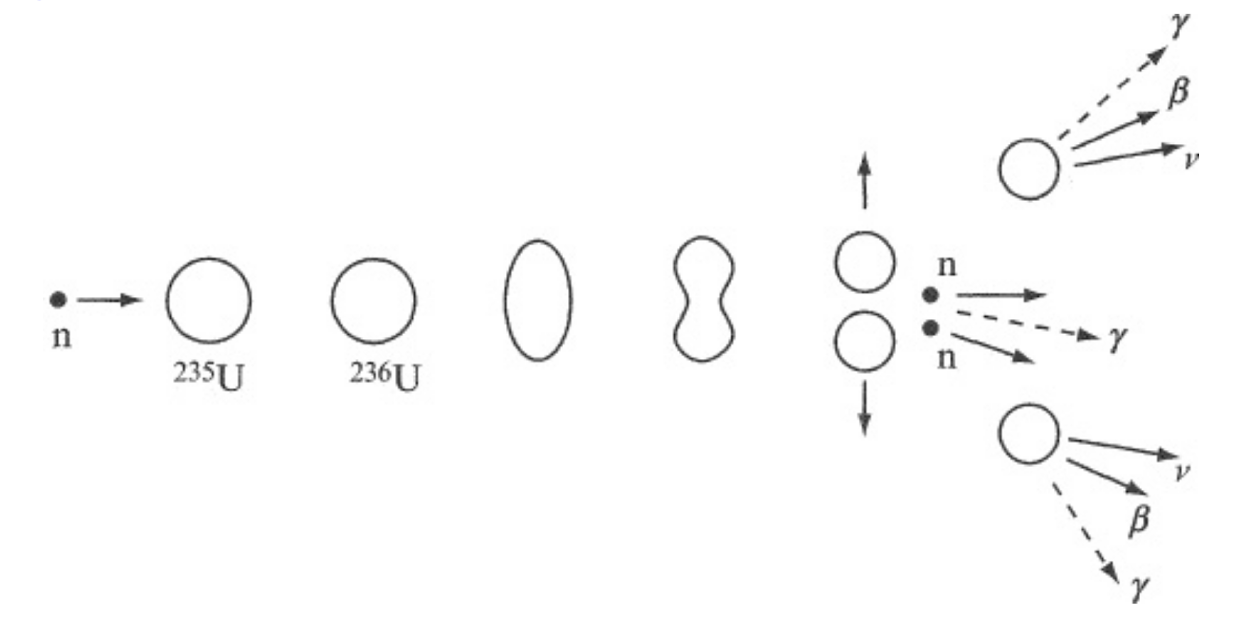
\includegraphics[width=0.8\textwidth]{fission.png}
            \caption{Illustration of the fission process for uranium-235.\cite{l01}}
            \label{fig:fission}
        \end{figure}

        \red{Wong has more on the fragmentation thing in his fission chapter.}

        \subsubsection{Fission energy budget}
        We can estimate the amount of energy released in fission by considering the binding energy difference
        and the properties of the product.
        The binding energy per nucleon is about $7.6$ MeV u${}^{-1}$ for uranium and about $8.5$ MeV u${}^{-1}$
        for a nucleus with atomic number around $117$. Hence, the change of binding energy per nucleon is
        $0.9$ MeV u${}^{-1}$, which amount to $212$ MeV for uranium-235.
        About $87\%$ of the total energy is promptly emitted because
        the fission products, carrying over $90\%$ of the total energy, travel for only a fraction of a
        millimeter before they are stopped. Besides, fission neutrons emit about $2$ MeV of energy by
        successive scattering in the reactor.
        About $13\%$ of the total energy goes into radioactivity. Energy carried by electrons and photons is
        convertible to heat but the neutrinos, carrying about $50\%$ of the radiation energy, are not stoppable.

        Henceforth, it is generally accepted that about $220$ MeV per fission is recoverable for energy conversion.
        The energy generated by the fission of uranium-235 is 
        about 2.5 million times the energy produced by burning coal of the same mass.\cite{e17}
        \subsubsection{Chain reaction??}

\section{Nuclear waste: classification and properties}
    \red{how much of each is generated and what the impact is; industry vs military}\\
    Different organizations have slightly different classification schemes for nuclear waste.
    However, their definitions of high-level waste (HLW), the most detrimental kind, are relatively consistent.
    The International Atomic Energy Agency (IAEA) classifies nuclear waste by considering the activity
    content and the half-life of the radionuclides (see FIG. \ref{fig:scheme}).
    Activity content is a measure of how much radioactivity
    a given amount of waste contains: a form of waste may possesses a high activity content due to
    \red{a high concentration of radionuclides or the presence of radionuclides with high activity.}\cite{iaea09}
    Each form of waste, depending on the half-life, activity content, and temperature, requires different
    disposal methods.
    \begin{figure}[h]
        \centering
        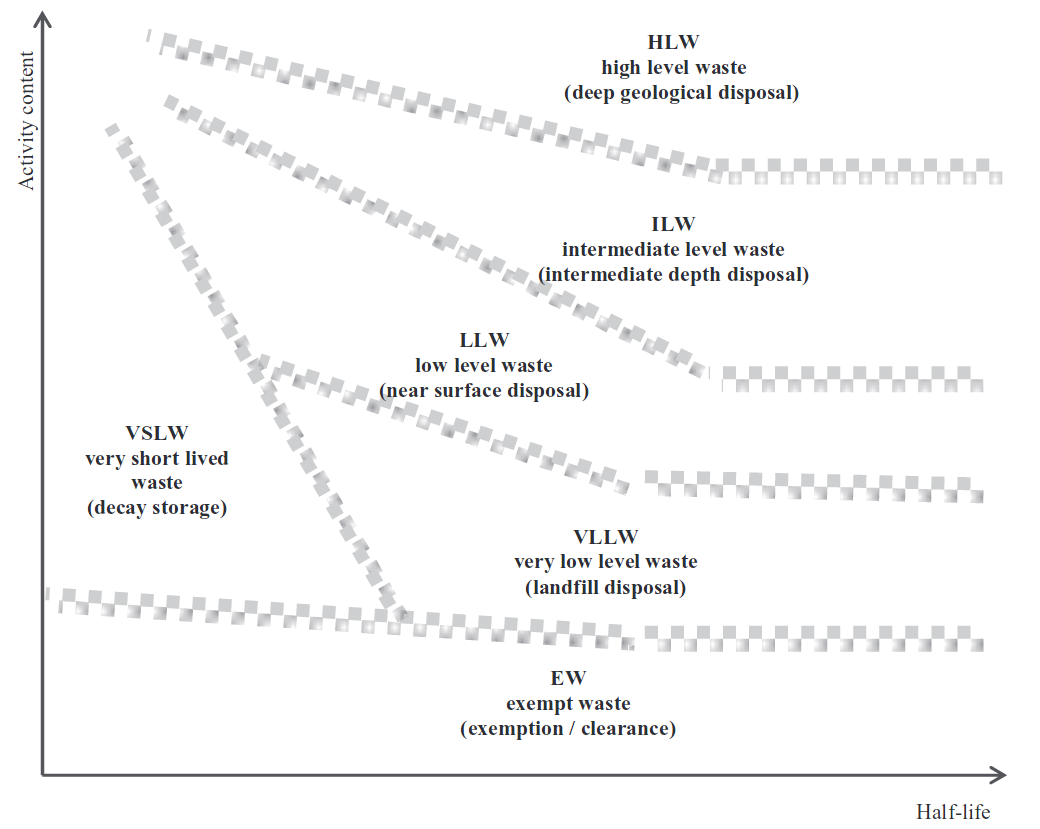
\includegraphics[width=0.7\textwidth]{wastescheme.png}
        \caption{An illustration of the IAEA classification scheme for nuclear waste along with suggested
        disposal methods.\cite{iaea09}}
        \label{fig:scheme}
    \end{figure}
    We will focus on high-level waste (HLW, defined below) in the rest of this work.
    In this section, we will first examine the composition and properties of HLW and then
    comment on other categories of waste and disposal methods.

    \subsection{High-level waste(HLW)}
    \red{reprocessing or not}\\
    \red{where does the heat come from?}
    High-level Wastes (HLW) has high activity contents and usually generates a large amount of
    heat as it radiates. The typical source of HLW is spent fuel from the nuclear reactor.
    In fact, since there is no commercial reprocessing facilities in the US (see section~\ref{sec:reproc}),
    almost all of the HLW is in the form of spent nuclear fuel from the reactor. In a nuclear reactor,
    fission of uranium-235 produces lighter radionuclides like cesium-137 and strontium-90, which
    account for most of the heat and penetrating radiation (\red{penetrating?}). In addition to
    the fission process, some uranium-235 atoms go through radiative capture
    (see section~\ref{sec:capture}) and produce elements that are
    heavier than uranium (``transuranic'') such as plutonium. The transuranic atoms do not generate
    as much heat or radiation as the fission products, but they tend to have a much longer half-life.
    For example, strontium-90 and cesium-137 have half-lives of about $30$ years, whereas
    plutonium-239 has a half-life of $24,000$ years.

    \subsection{Transuranic waste(TRU)}
    Transuranic waste is defined as materials that do not belong to high-level waste and are
    contaminated by alpha-emitting radionuclides with
    sufficiently long half-life ($<20$ years) of elements with atomic number $92$ (atomic number of uranium)
    or larger and concentration of activity larger than $3700$ Bq/g.\cite{j83,s01}. The activity
    of TRU is usually low but it remains active for long period of time.
    \red{WIPP is only for TRU}

    \subsection{Low-level and intermediate-level waste (LLW and ILW)}
    Low-level waste (LLW) has relatively little radioactivity, produces almost no heat,
    and contains practically no
    transuranic elements. Examples are papers and tools used in cleanup operations in the reactor.
    Most LLW does not require shielding and may be buried in landfill 
    facilities after on-site short-term decay storage.
    Some LLW (for example, metal nuclear fuel cladding) may have a slightly
    higher radioactivity such that they are classified
    as intermediate-level waste (ILW). ILL are solidified in concrete and buried in shallow
    repositories.\cite{s01} However, US regulations do not make the distinction
    between LLW and ILW but different disposal methods are practiced.\cite{nrc09, s01}

    \subsection{Uranium tailings}
    Uranium mill tailings from uranium mills are another form of waste with low activity, but
    they are not usually classified as LLW. The tailing is what is left after the uranium has been
    extracted from the ore. The decay of uranium-238 from the mill decays into
    radioactive thorium and radium and these radionuclides stay in the tailing. Notably, radium
    can decay into radon gas which is an alpha-emitter. Hence, the alpha radiation can do additional
    damage to body if the radon enters the body as one breathes.
    The uranium tailings leave the uranium mills in the form of a liquid sludge
    and can dry. Therefore, it is necessary to prevent the uranium tailings
    from contaminating water and air.
    
    \section{Spent fuel management}
    Spent fuel from nuclear reactors constitutes the major source of HLW. Spen fuel pools at the
    reactors hold spen fuel cores to cool them down and isolate them for a few years. After that,
    reprocessing can occur to extract the most radioactive plutonium and uranium isotopes and
    convert the waste into more managable form (vitrification). However, reprocessing of commercial
    nuclear spent fueld did not
    happen in this country for various historical reasons. 
    \subsection{Spent fuel pools}
    \red{boron-10 and radiation shielding.}
    The heat output of the spent fuel decreases by $99\%$ after the first year and by another factor of $5$
    by the 5-year mark.\cite{aa12} Therefore, short-term cooling of spent fuel is crucial before
    futher disposal or reprocessing can be done.
    US nuclear power plants generally have an operation cycle of about 2 years. At the end of each operation cycle,
    one-quater to one-third of its fuel assemblies (spent fuel) are removed. The removed spent fuel spend a minimum
    of five years in these water pools to cool.
    Most of the nuclear industry's spent fuel is now stored in spent fuel water pools ``at-reactor (AR)'',
    which means either within the reactor building or in an ajacent spent fuel building linked to the reactor
    AR pools minimize the difficulty of transporting spent fuel.\cite{iaea99}
    US has generated about $65,000$ metric tons of spent fuel, of which $75\%$ is stored in AR pools.\cite{a11}
    by a transfer tunnel. 
    Spent fuel pools  are usually about 15-meter deep water pools, with storage rack at the bottom to hold the fuel assemblies.
    The water absorbs the heat and shields the radiation. Water is the chosen medium because it is cheap and
    can provide coooling by circulation. Moreover, water can serve as a shielding from radiation, because it has a
    fairly high density and hence forces the radiated particles (especially the neutrons) to interact with
    the water molecules and lose energy \red{(more precise terms needed, cladding materials)}. Water temperature is maintained
    below 50 $^\circ$C via circulation and cooling. The integrity of the storage can persist well beyond 
    50 years.\cite{a11, iaea99}

    \subsection{Reprocessing: an option}
    \label{sec:reproc}
    After spending some time in the nuclear fuel pools and cooling down, the spent fuel may be ready
    for reprocessing.
    Spent nuclear fuel contains a large amount of plutonium and uranium that are suitable as nuclear fuel
    or fissile weapon material (plutonium-239). Therefore, reprocessing the spent fuel generates plutonium and
    uranium that may be recycled. The US currently does not have any commercial nuclear fuel
    reprocessing facility due to the demonstrated high cost of reprocessing
    during the West Valley Demonstration Project and water contamination issues at the Hanford Site.
    Concerns about proliferation issues also arise, as the 
    reprocessed plutonium-239 is the primary fissile element in the production of nuclear weapons.\cite{aa12}
    On the other hand, France (the world leader in reprocessing technology), India, Japan, Russia, the UK
    and China (since 2010) continues to reprocess spent fuel. To understand the details of reprocessing
    requires advanced chemistry and is beyond the scope of this work. However, the issue remains interesting
    and hence we provide an overview of the process as well as some of the related concerns.

    Almost all of the reprocessing plants use the PUREX (Plutonium Uranium Redox EXtraction) process
    to reprocess spent fuel. This process utilizes the differences in oxidation potential 
    between the heavy elements (uranium and plutonium) from the other lighter fission products.
    The process involves three steps: (a) adding appropriate solvent (usually nitric acid) to absorb and oxidize 
    plutonium and uranium while leaving out other elements;
    (b) adding a reducing (de-oxidizing) agent that reduces (de-oxidizes) only the
    oxidation state of plutonium to one that is insoluble
    and thus seperable; and finally (c) extracting the plutonium from the mixture. In this way
    the oxidized plutonium and uranium are separated and can be reduced back to reusable radionuclides.\cite{lb01} 
    The extracted plutonium then returns to the reactor and transforms into short-lived fission products
    by fission. Un-reprocessed fuel usually takes 10 times as much time to reach the safe
    activity level (\sim$10^5$ years) as reprocessed fuel (\sim$10^4$ years). Moreover, since fission products
    make up a small portion of the spent fuel, reprocessing greatly reduces the mass of the waste. The reprocessed
    waste can be turned into liquid form, mixed with frit (the substance from which glass is made) and then
    vitrified (made into glass). The vitrification process immobilizes the radioactive particles and makes
    the waste much more safe and manageable, but vitrification can only be applied to reprocessed spent fuel.

    It is worthwhile to note that the PUREX processed was designed specifically to seperate plutonium for
    bombs. Therefore, literally any other reprocessing approach would be less prone to proliferation.
    Researchers are actively investigating alternatives to the PUREX technology. For example, the UREX+ (for
    uranium extraction) technique extracts the uranium but leaves the plutonium mixed with other
    radioactive materials. Another popular alternative, pyrochemical reprocessing, inserts giant electrodes
    into the chemical bath of nuclear waste and electroplates the plutonium and other transuranics onto
    the electrode. However, none of these alternatives have been put into practice due to the high construction
    and operating costs of reprocessing facilities.\cite{aa12}

    \red{fast neutron reactors}

    \subsection{Dry cask storage}
    Spent fuel pools have very limited capacities. 
    Overground dry cask storage provides a low-cost temporary storage before the spent fuel is disposed of.
    After cooling in the spent fuel pools for a few
    years, the spent fuel can be stored in dry casks filled with inert gas. 
    The dry casks are often metal cyliders welded to prevent leakage. Each cask is surrounded by
    additional steel and concrete to provide shielding.
    The heat from the cask is removed by passive
    cooling (air circulation). The Nuclear Regulatory Comission is hoping that the casks will
    last safely for as long as 100 years, yet corrosions and cracking occur in 30 years
    or less.\cite{aa12} As such, without the prospect of a permanent geological repository,
    overground dry cask storage does not seem to be a long-term solution. The doubts were expressed
    dudring  the Nuclear Waste Technical Review Board 2009 meeting \cite{nwtb09, aa12}
    \begin{displayquote}
    Leaving the spent fuel onsite for extended periods of time was never intended and is not
    responsible. (Dry cask manufacturer)

    It is not ethical, basically to plan for long-term storage without pursuing a well defined repository
    program. (Department of Energy employee speaking as a citizen)
    \end{displayquote}
    Even more striking is the fact that more than $75\%$ of the spent fuel are still stored in pools
    that are close or over to their designed limits.\cite{a11,aa12}
    Therefore, there is clearly a need for a long-term disposal plan, which we will epxplore in
    the next section.\\
    \red{(A lot more drama with the NRC going on here, loss of credibility.)}

\section{Disposal of HLW}
    The timeframe of nuclear waste disposal is about $10^4-10^6$ years, after which the radioactivity
    of the waste decreases down to a safe level.
    Deep geological repositories that are stable over timescales naturally offer a good option for disposal.
    It is accepted that geological repositories in a stable environment over 300 meters below ground
    is safter than indefinite overground storage of HLW, reprocessed or not.\cite{fmr11}
    
    Reversible repositories hm.
%    \subsection{Comments on partitioning and transmutation}
    \subsection{Requirements for HLW disposal}
     \subsection{Survey of possibilities}
     transmutation, ocean floor, deep geological disposal
%    \subsubsection{mention ocean disposal and why it was banned('Ndrangheta)}
%    \subsection{Necessity of geological disposal sites}
%    \subsection{Requirements of disposal from physics}
     \subsection{Deep borehole disposal}
     \subsection{Deep geological repository}
%
\section{Deep Geological Repository}
    Therefore, long-term storage before final disposal is crucial. 
    \subsection{something general}
    \subsection{Yucca Mountain}
    \subsection{Something related to the French Ciegeo project: licensed reversible disposal site}
    \subsection{Risk calcs: geophysics, mention WIPP}

\section{Discussions}

k
\begin{acknowledgments}
Thanks Joel and peeps. Arjendu and M. V. Ramana.
\end{acknowledgments}

\pagebreak
\bibliographystyle{aip}
\bibliography{refs}
\appendix
\section{Derivation of Fermi's Golden Rule \#2}
\label{a:fermi}
\end{document}
